\chapter{The application}
\section{Overview of the requirements}
As mentioned in the 2nd chapter of the thesis, one of the major problems in many applications that revolve around permissions is the fact that they don't provide a granular enough system. In order to deal with this, unlike the Google Drive, the demo application must implement an exhaustive system, and unlike unix systems, the application must allow multiple roles to be assignable to a single user.

In order to achieve this the application must have the following features:
\begin{itemize}
    \item A user system, and therefore the ability to switch between the perspective of different users.
    \item A way of managing roles: assigning roles to users, changing permissions of the roles, adding/removing roles.
    \item And finally, a way of actually testing the permissions out in a realistic environment.
\end{itemize}

\section{Backend --- used technologies}
\subsection{.NET and C\#}
.NET is a free, cross-platform and open source framework developed by Microsoft, that started as proprietary. The reason .NET was chosen for this application is because it provides an environment for building very expandable Rest APIs. 

One of the key benefits of .NET core is Entity Framework Core. Entity Framework (EF) Core is a lightweight, extensible, open source and cross-platform version of the popular Entity Framework data access technology.

EF Core can serve as an object-relational mapper (O/RM), which\cite{efCore}:

\begin{itemize}
 	\item Enables .NET developers to work with a database using .NET objects. \item Eliminates the need for most of the data-access code that typically needs to be written.
\end{itemize}

EF Core supports many database engines such as SQLite, PostgreSQL, MySQL, etc.
\subsection{LINQ}
LINQ or Language integrated query is the name for a set of technologies based on integrating SQL-like queries straight into C\#, which has the benefit of compile-time checking rather than runtime. Writing SQL code as a set of string is very error prone and fairly hard to manage, and LINQ helps to alleviate that problem.

To do that, LINQ provides SQL-specific keywords such as \verb|from|, \verb|where|, \verb|select| which can be used on collections as shown in figure \ref{FigLINQExample}.

\begin{figure}[htbp]
	\centering
		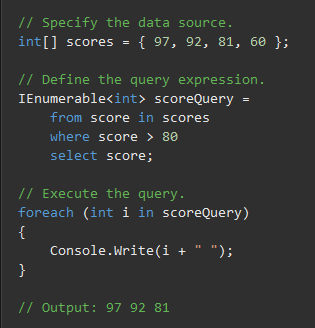
\includegraphics[scale=0.85]{./figures/chapter4/linq_example.png}
	\caption{LINQ Example}
	\label{FigLINQExample}
\end{figure}

The LINQ system further contributed to the choice of using .NET for the application, since there were a lot of interconnected entities.

\subsection{JSON Web Token}
Even though the scope of this thesis is to explore the permission management in an application focused on collaborative content viewing, it would all be futile if the application is easily exploitable through security vulnerabilities, and thus a need for a secure and encrypted means of communication between the front end and the back end exists.

The JSON Web Token or JWT for short is a proposed internet standard for creating data with optional signature and/or optional encryption whose payload holds JSON that asserts some number of claims.
\section{Frontend --- used technologies}
\subsection{React.js}
React (also known as React.js or ReactJS) is a free and open-source front-end Java-Script library for building user interfaces based on UI components. It is maintained by Meta (formerly Facebook) and a community of individual developers and companies.

React is component based which allows the user to build encapsulated components that manage their own state, and then further compose them into a more complex user interface.

React also makes it painless to create interactive UIs. Design simple views for each state in your application, and React will efficiently update and render just the right components when your data changes. \cite{reactJs}

Declarative views make your code more predictable and easier to debug.

\subsection{Typescript}
TypeScript is a programming language developed and maintained by Microsoft. It is a strict syntactical superset of JavaScript and adds optional static typing to the language. It is designed for the development of large applications and transpiles to JavaScript. As it is a superset of JavaScript, existing JavaScript programs are also valid TypeScript programs. 

TypeScript provides static typing through type annotations to enable type checking at compile time. This is optional and can be ignored to use the regular dynamic typing of JavaScript. 

Because Typescript provides typing, developing becomes overall easier as code is much easier to debug since you won't rely on runtime errors to spot bugs, but instead, the code fails at compile time.

\subsection{Material UI}
The main reason react was chosen lies within the material ui library. MUI is a ReactJS library that provides components based on the Material UI standard developed by Google. It allows a quick and easy way of developing responsive applications without the need of worrying about the aesthetic of the application.

The components that it provides also come with a lot of functionality by default which further saves time during development.


\section{Software Requirements}
In order to run both the projects, an operating system is needed. Due to the fact that the backend project uses .NET, the software requirements regarding the operating system are mostly given by it. Hence a machine with an operating system that can run dotnet CLI at minimum is needed. 

Known supported operating systems include\cite{dotnetSupportedOs}:
\begin{itemize}
    \item Windows and Windows server
    \item MacOS
    \item Linux and linux servers: Ubuntu, Alpine, CentOS, Debian, etc.
\end{itemize}

For the frontend the major dependency is React.js, in order to install that Node.js is needed. 

The operating system requirements for nodejs are pretty much the same as the ones for dotnet\cite{nodejsSupportedOs}:
\begin{itemize}
    \item Windows
    \item MacOS
    \item Linux: Ubuntu, Debian, CentOS, etc.
\end{itemize}

Since both projects are essentially source code that needs to be compiled, an IDE (Integrated Development Environment) is strongly recommended for both of them.

For the backend project there are many different choices: Rider, Visual Studio, Visual Studio Code. As for the frontend project, any IDE that has support for html, css, typescript should suffice, for example InteliJ, PhpStorm, WebStorm, Visual Studio Code, Sublime Text.

During the development phase, I used Rider for the backend and PhpStorm for the front end, which I strongly recommend as that is what will be used to explain the setup and running of the projects.

\section{Setup}
Since the application is split into two different projects, each one of them needs to be set up individually.
\subsection{Backend}
The backend is written in C\# with .NET framework core. The first requirement is to have dotnet installed. After that the app settings need to be configured. To do that, navigate to \verb|Backend/Backend|, and copy paste the template file called \verb|appsettings.template.json| into another file called \verb|appsettings.json|.

\begin{figure}[htbp]
	\centering
		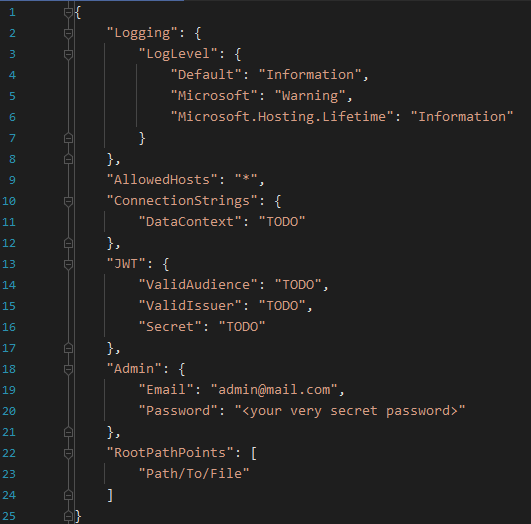
\includegraphics[scale=0.85]{./figures/chapter4/appsettings_template.png}
	\caption{App settings template}
	\label{FigAppSettingsTemplate}
\end{figure}

Next, as shown in figure \ref{FigAppSettingsTemplate}, a few fields need to be filled. The first field is related to the \verb|ConnectionStrings|. A ConnectionString is a way of specifying how to connect the application to the database. During development, the database used was SQLite. 

To specify a connection to that set \verb|DataContext| equal to \\ \verb|"Data Source=<Location>;"|, where Location will be the location of the \\ database. 

Example: \verb|"DataContext":  "Data Source=Kumo.db;"|.

The second field that needs to be configured is related to the JSON Web Token  (JWT). The ValidAudience represents the location at which the requests with the token will be valid. For example if you want to have only one computer use the API, then the IP address of that computer will become the ValidAudience, meanwhile in the case where anybody can be a valid audience, the field is set to \verb|*|. Next, the ValidIssuer represents the location from which the token can be created. This is always the address associated with the server.

The final and the most important field from the JWT configuration is the \verb|Secret|. This represents a base64 encoded string which is used for creating the token. If this field is not secure enough, or it gets leaked, then the JWT becomes reversible, which is why this field is extremely important to remain a secret.

The third field that needs to be configured is related to the Admin. Normally having an endpoint that creates an administrator user is bad practice, which is why the application handles this by providing a way of creating the administrator user at the first start of the application. The \verb|Email| and \verb|Password| fields are explanatory.

The fourth field is related to the Root Path Points. In short, a root path point is a place from which the navigation can start. This field is not mandatory as these can be created from the front end, via the administrator account.

After setting up the \verb|appsettings.json| file, the next step is to create the database and all of the schema for it. To do that, we need to run migrations which require a dependency called \verb|dotnet-ef|. 

To install \verb|dotnet-ef|, a few commands need to be run. The first one being \verb|dotnet tool install --global dotnet-ef|. After that we can create the database, to do that you need to be in the same directory as the \verb|appsettings.json| file, and then run \verb|dotnet ef database update|.

With that, all the setting up for the back end is finished, and the backend is now runnable.

Open your IDE of choice, in this case Rider will be used. Simply open the project in it, and hit the \verb|Run| button in the top right corner.

\begin{figure}[htbp]
	\centering
		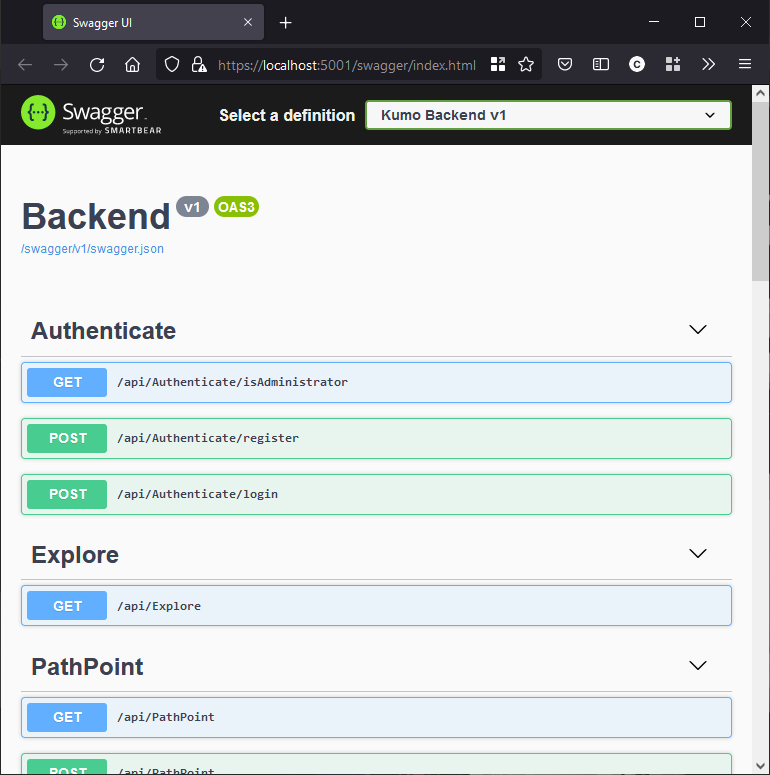
\includegraphics[scale=0.6]{./figures/chapter4/backend_swagger.png}
	\caption{Swagger and the API endpoints}
	\label{FigBackendSwagger}
\end{figure}

After that, you should see Swagger, like shown in the figure \ref{FigBackendSwagger}.

\subsection{Frontend}
Compared to the backend project, setting up the frontend is significantly easier, as only two commands need to be run. After navigating to the \verb|frontend| directory, we need to install the dependencies. To do that simply open a terminal and write \verb|npm install|.

After that completes, open your IDE of choice, in this case PhpStorm will be used. Open the project in it and then run it via the \verb|Run| button.

\begin{figure}[htbp]
	\centering
		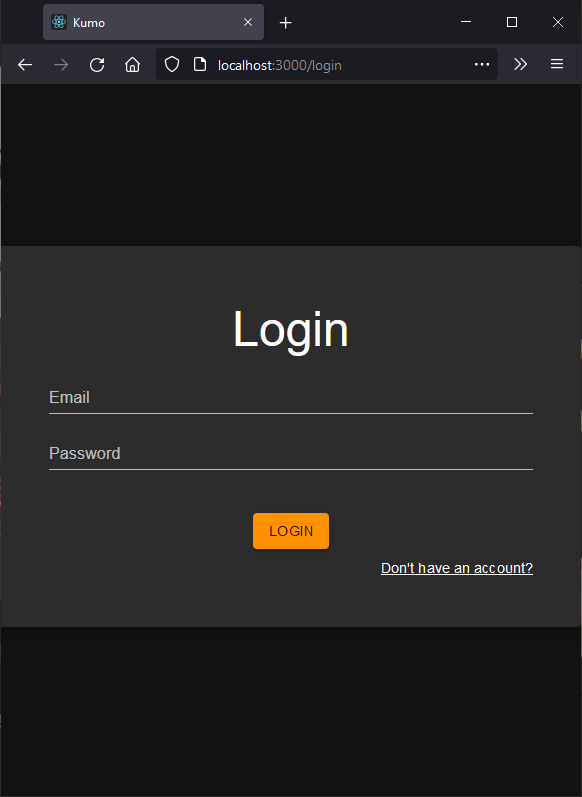
\includegraphics[scale=0.5]{./figures/chapter4/frontend_login.png}
	\caption{Frontend login page}
	\label{FigFrontendLogin}
\end{figure}

Once the application has finished compiling, a browser will open and you will see a login screen, as shown in \ref{FigFrontendLogin}.


\section{Implementation details}
The implementation of the application uses RBAC, hence a way of managing roles is needed. This however starts with correctly separating the data in the database to make different operations possible and to account for different use cases.

To do this the data is structures into 6 classes:
\begin{itemize}
	\item PathPoint --- represents a specific location, has one important property: \verb|isRoot|. \verb|isRoot| represents if the path should be displayed on the explorer's home page;
 	\item FileSystemEntryType --- an enum that specifies if the system entry type is a file or a folder, or unknown;
	\item Role --- self explanatory, it represents a role;
	\item Permission --- this is an n:m relation between a PathPoint and a Role, with additional data such as: Read, Write, Delete;
	\item User --- this represents a user in the application;
 	\item UserRole --- this is an n:m relation between a User and a Role.
\end{itemize}

\section{Application usage}
As mentioned in the requirements, in order to explore the problem of permissions, 3 main functionalities are needed. A way of managing users, a way of managing permissions, and a real life usage of those permission.
\subsection{Users}
Thus, the first requirement the application must have is a way of handling users. The application has functionality for register\ref{FigFrontendRegister}, login\ref{FigFrontendLogin}, and logout marked with a (1) in \ref{FigFrontendLogout}.

\begin{figure}[htbp]
	\centering
		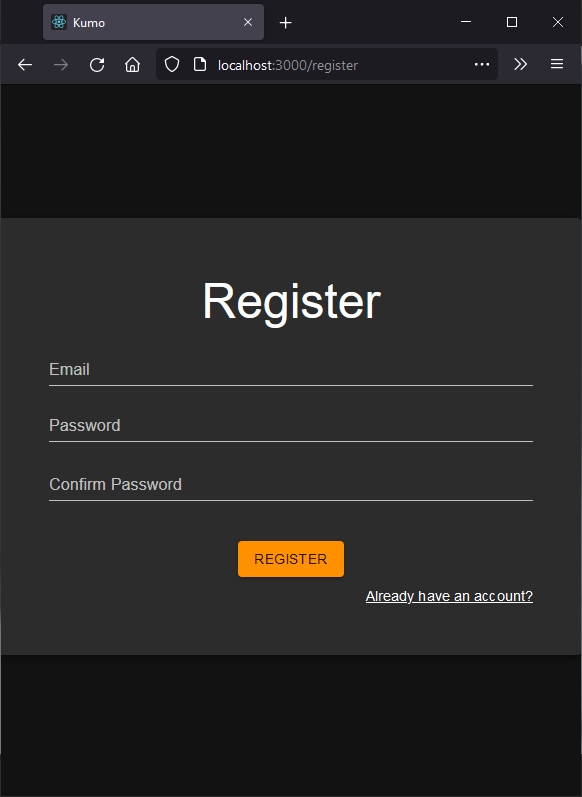
\includegraphics[scale=0.5]{./figures/chapter4/frontend_register.png}
	\caption{Frontend register page}
	\label{FigFrontendRegister}
\end{figure}

\begin{figure}[htbp]
	\centering
		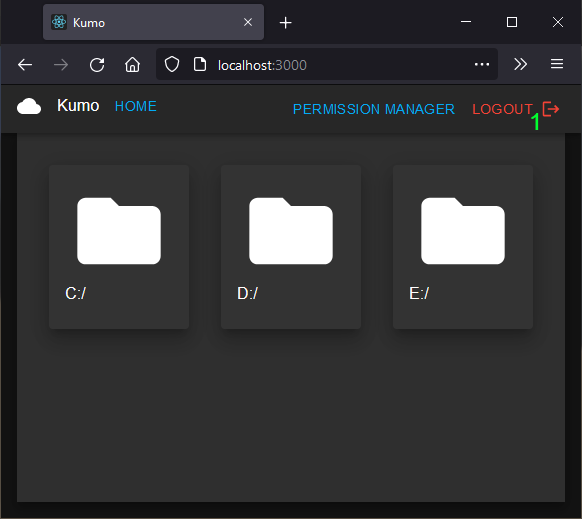
\includegraphics[scale=0.5]{./figures/chapter4/frontend_logout.png}
	\caption{Frontend logout functionality on the main page}
	\label{FigFrontendLogout}
\end{figure}

Being trivial functionality, there is no reason to go over the flow of each of the actions.
\subsection{Explorer}
The real life usage of the permissions is an Explorer. The explorer, essentially, provides a way of navigating folders on a hard drive.

Being used as a proof of concept, the main purpose of the explorer is to give a visual representation of how the "Read" permission works across all instances where it has been set. Due to the fact that the permission system takes into account permissions such as "Delete" and "Write", the Explorer can be easily expanded to accommodate for those too, however for the sake of example the Read permission will be used as a visual representation, while the response from the API calls will contain more information.

\begin{figure}[htbp]
	\centering
		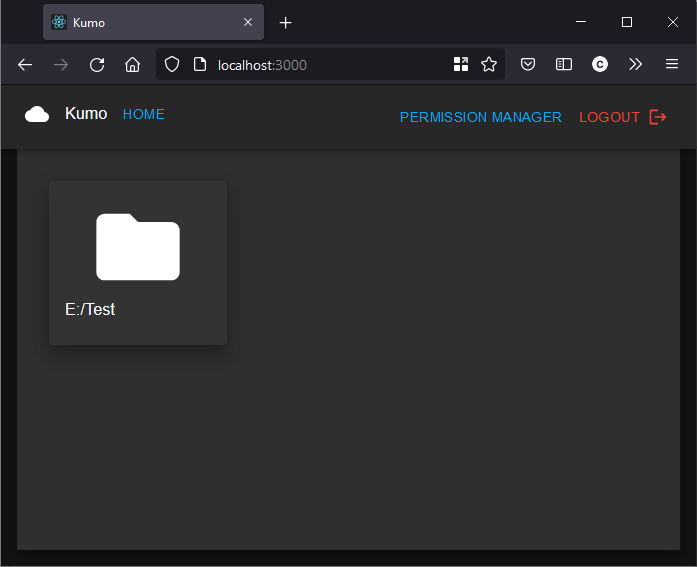
\includegraphics[scale=0.65]{./figures/chapter4/explorer_home.png}
	\caption{Explorer home path}
	\label{FigExplorerHome}
\end{figure}

\begin{figure}[htbp]
	\centering
		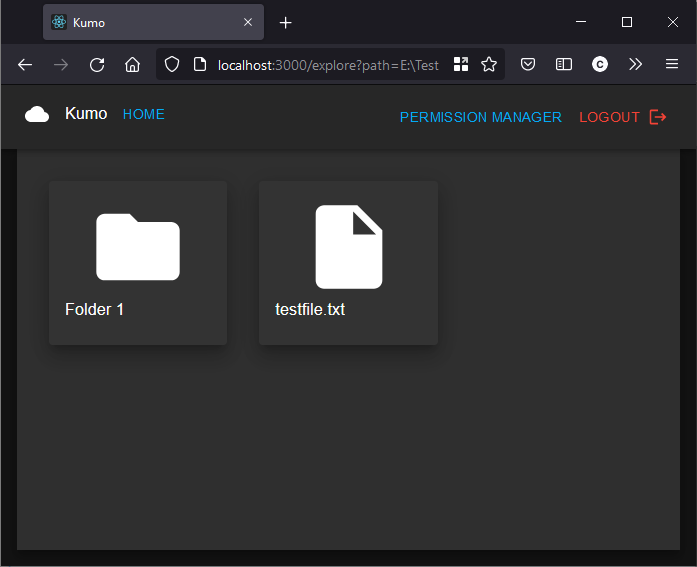
\includegraphics[scale=0.65]{./figures/chapter4/explorer_subfolder.png}
	\caption{Explorer subfolder navigation}
	\label{FigExplorerSubFolder}
\end{figure}

As mentioned in the implementation details, on the explorer home page\ref{FigExplorerHome} the root path points are shown. When a user clicks on a directory, the explorer moves inside that subdirectory and shows the files and folders inside it. When clicking on the \verb|E:/Test| subfolder it's contents are shown as in \ref{FigExplorerSubFolder}.

\subsection{Permission management}
The most important part of the application is the permission management system. As mentioned in Setup of the Backend, an admin account is needed. To properly show the functionality of this, I'm going to use two browsers which are connected to two accounts. As shown in \ref{FigPermissionManagerButton}, the browser on the left is connected to an admin account, which shows the \verb|PERMISSION MANAGER| button, while the browser on the right doesn't.

\begin{figure}[htbp]
	\centering
		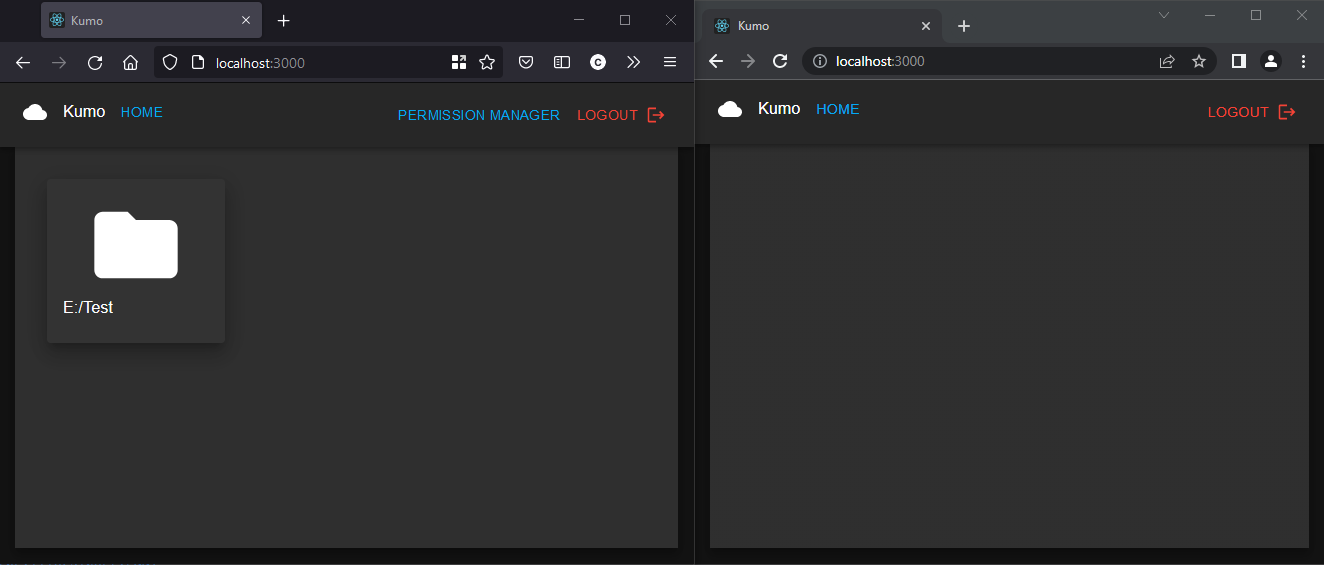
\includegraphics[scale=0.4]{./figures/chapter4/explorer_permission_manager.png}
	\caption{Permission manager button on an admin account and on an normal account}
	\label{FigPermissionManagerButton}
\end{figure}


You'll notice that in figure \ref{FigPermissionManagerButton}, the user on the right does not see any path points. And that is because there are no permissions configured yet aside from the \verb|E:/Test| path point.

To configure the permissions, the first step is to go to the Permission Manager. Due to the complexity of the permission manager, there are 4 configurable entries as shown in figure \ref{FigPermissionManagerHome}

\begin{figure}[htbp]
	\centering
		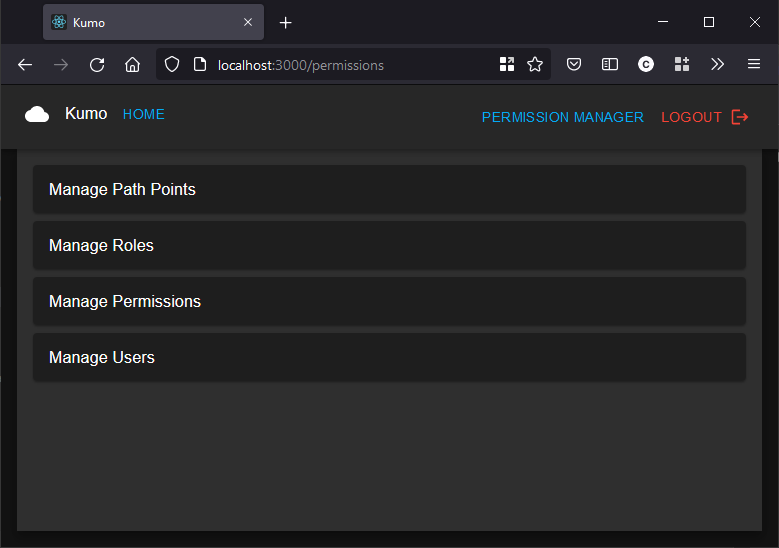
\includegraphics[scale=0.6]{./figures/chapter4/permission_manager_home.png}
	\caption{The default view of the permission manager}
	\label{FigPermissionManagerHome}
\end{figure}

To demonstrate the power of the permission system, we will configure the scenario mentioned in chapter 2, the hard to express file structure from google drive shown in figure \ref{FigDriveBadScenario}.

\subsubsection{Configuring Path Points}
Once you click on the \verb|Manage Path Points| button, the accordion will expand and the path point manager will be shown as in figure \ref{FigPermissionManagerPathPoints}

Firstly, all managers have a table that show the entries available in the database. In the case of the Path Point Manager, there are a number of important elements:
\begin{itemize}
	\item (1) --- Shows the path of the path point
	\item (2) --- Shows whether or not the path point is root
	\item (3) --- Marks the entry for deletion
	\item (4) --- Commits the changes from the table to the database
	\item (5) --- Cancels all of the changes and reverts to the original state from the database
	\item (6) --- The path of the new path point to be added
	\item (7) --- Whether or not the path point is a root path point
	\item (8) --- Adds the path point to the database
\end{itemize}

Entries (1) and (2) can be edited by double clicking on them.

To achieve the file structure mentioned, where the Sensitive Data isn't accessible by a user, a path point that is not a root is needed for the \verb|Sensitive Data| folder as shown in figure \ref{FigPermissionManagerPathPointsCorrect}.

\begin{figure}[htbp]
	\centering
		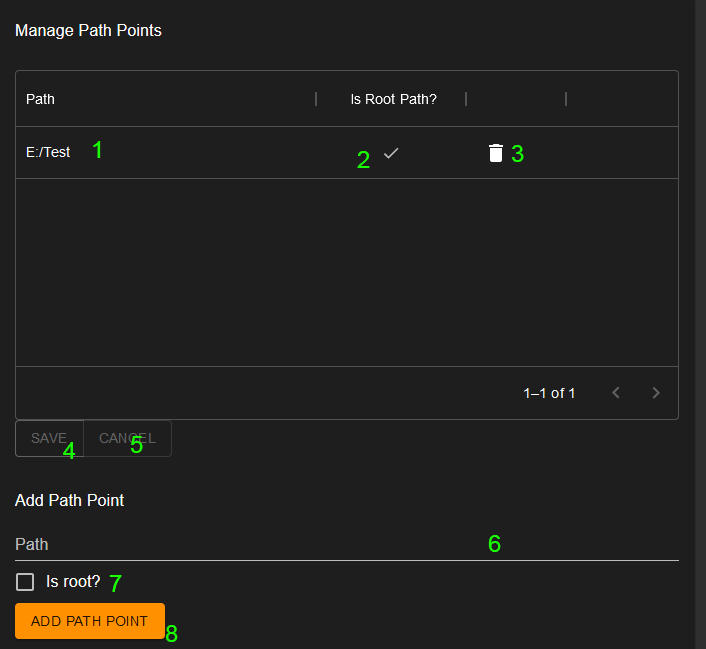
\includegraphics[scale=0.5]{./figures/chapter4/permission_manager_path_points.png}
	\caption{Path point manager}
	\label{FigPermissionManagerPathPoints}
\end{figure}


\begin{figure}[htbp]
	\centering
		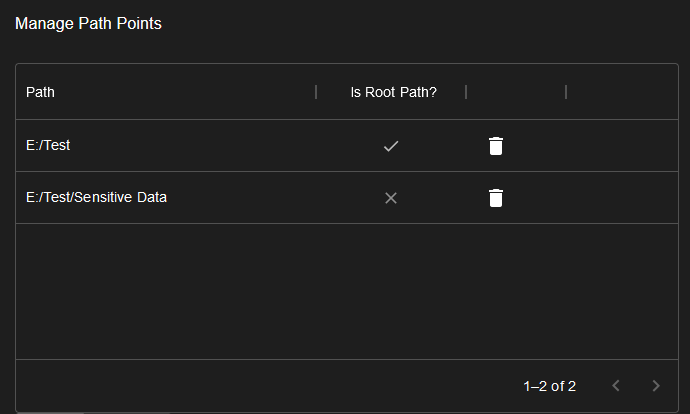
\includegraphics[scale=0.65]{./figures/chapter4/permission_manager_correct_path_points.png}
	\caption{The correct path point structure needed}
	\label{FigPermissionManagerPathPointsCorrect}
\end{figure}

\subsubsection{Configuring Roles}
To achieve the desired permission structure only one role is needed, to do that configure it by opening the role manager as shown in \ref{FigPermissionManagerRoles}.

The important elements in the role manager are as follows:
\begin{itemize}
	\item (1) --- The name of the role;
	\item (2) --- Marks the element for deletion;
	\item (3) --- Commits the changes from the table to the database;
	\item (4) --- Cancels all of the changes and reverts to the original state from the database;
	\item (5) --- The name of the role to be added;
	\item (6) --- Adds the role to the database.
\end{itemize}

\begin{figure}[htbp]
	\centering
		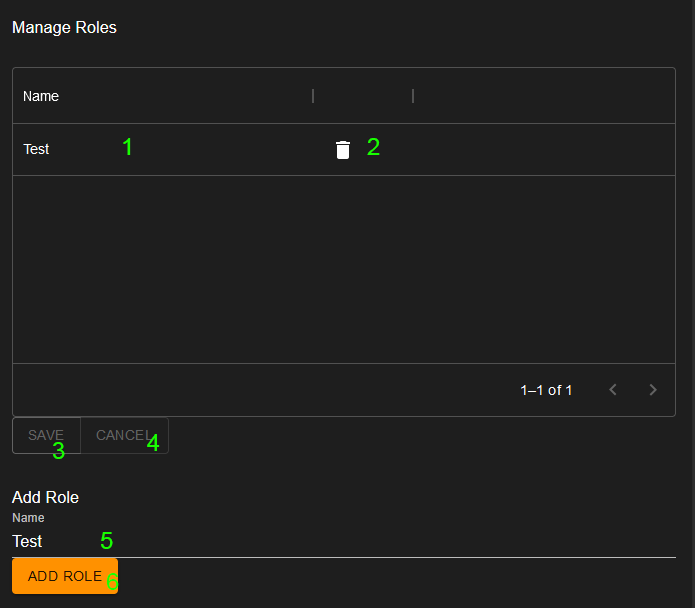
\includegraphics[scale=0.5]{./figures/chapter4/permission_manager_roles.png}
	\caption{Roles manager}
	\label{FigPermissionManagerRoles}
\end{figure}

\subsubsection{Configuring Permissions}
For configuring permissions we essentially need to specify that the \verb|E:/Test| path is readable by the \verb|Test| role, and the \verb|E:/Test/Sensitive Data| is not readable by the \verb|Test| role.

As marked in figure \ref{FigPermissionManagerPermission}, the important elements are as follows:
\begin{itemize}
	\item (1) --- The role for which the permission is applied;
	\item (2) --- The path for which the permission is applied;
	\item (3), (4), (5), (6) --- Whether or not the role can: Modify Root, Read, Write, or Delete;
	\item (7) --- Marks the element for deletion;
	\item (8) --- Commits the changes from the table to the database;
	\item (9) --- Cancels all of the changes and reverts to the original state from the database;
	\item (10) --- The role of the new permission
	\item (11) --- The path point for the new permission
	\item (12), (13), (14), (15) ---  Whether or not the new role can: Modify Root, Read, Write, or Delete;
	\item (16) --- Adds the permission to the database.
\end{itemize}

\begin{figure}[htbp]
	\centering
		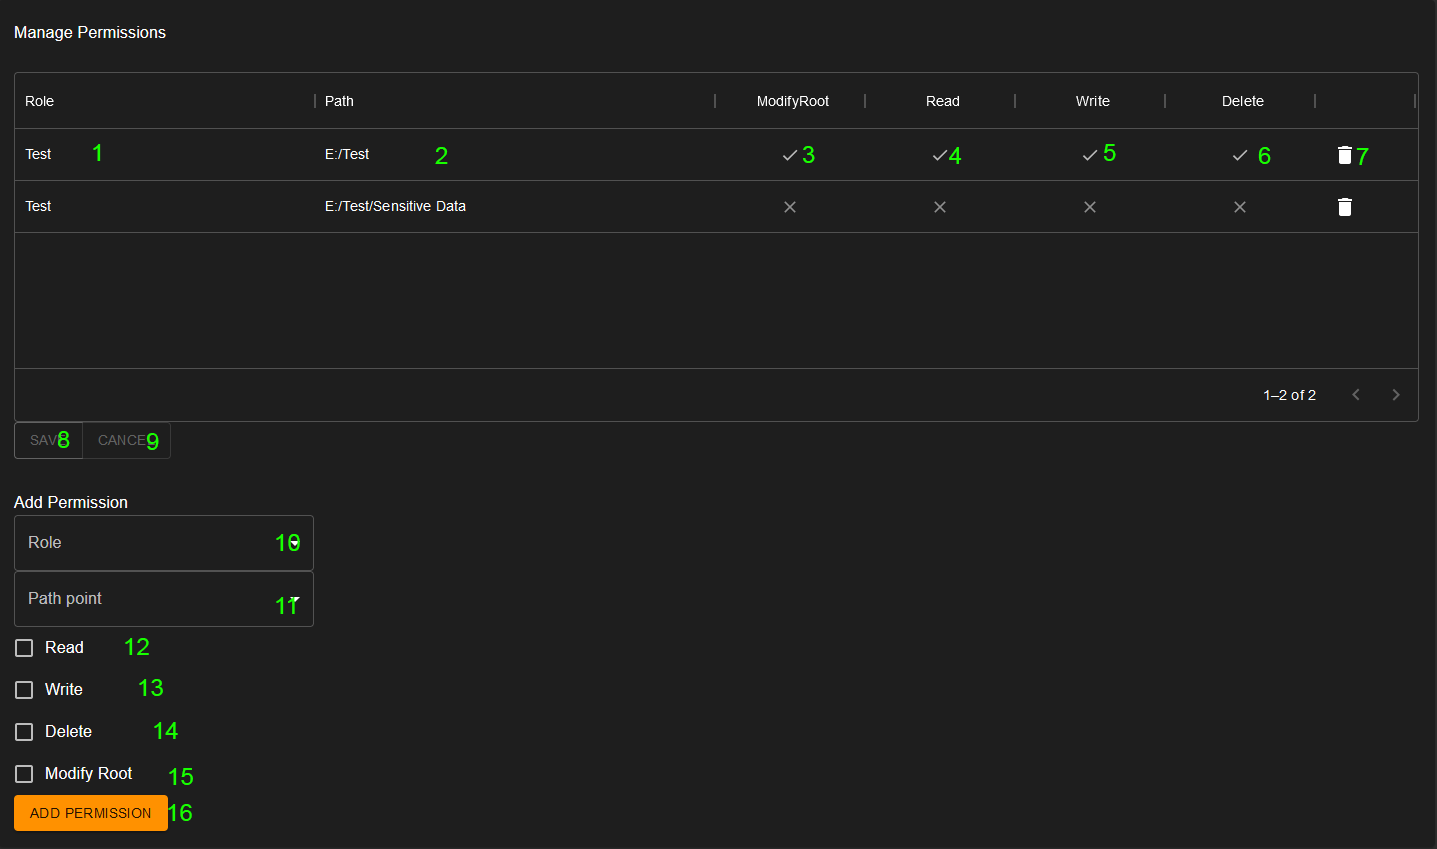
\includegraphics[scale=0.3]{./figures/chapter4/permission_manager_permission.png}
	\caption{Permission manager}
	\label{FigPermissionManagerPermission}
\end{figure}


\subsubsection{Configuring Users}
The last step is to connect the \verb|test@mail.com| user to the \verb|Test| role.

As marked in figure \ref{FigPermissionManagerUser}, the important elements are as follows:
\begin{itemize}
	\item (1) --- The user that is linked;
	\item (2) --- The role to which the user is linked;
	\item (3) --- Marks the element for deletion;
	\item (4) --- Commits the changes from the table to the database;
	\item (5) --- Cancels all of the changes and reverts to the original state from the database;
	\item (6)--- The user that will be linked;
	\item (7) --- The role the user will be linked to;
	\item (8) --- Links the user to the role in the database.
\end{itemize}

\begin{figure}[htbp]
	\centering
		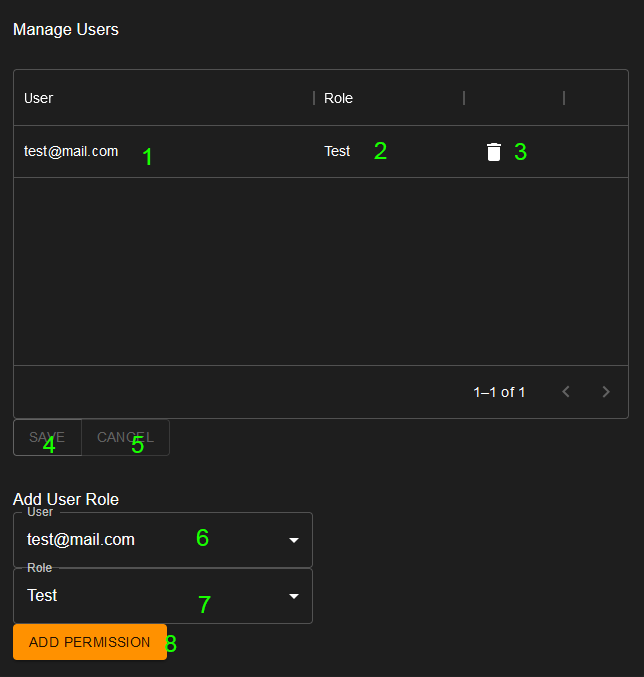
\includegraphics[scale=0.5]{./figures/chapter4/permission_manager_users.png}
	\caption{User manager}
	\label{FigPermissionManagerUser}
\end{figure}

With that all of the configuration has been done, if the user \verb|test@mail.com| navigates to the \verb|E:/Test| path, they will be unable to see the \verb|Sensitive Data| directory, as shown in figure \ref{FigPermissionManagerResult}.


\begin{figure}[htbp]
	\centering
		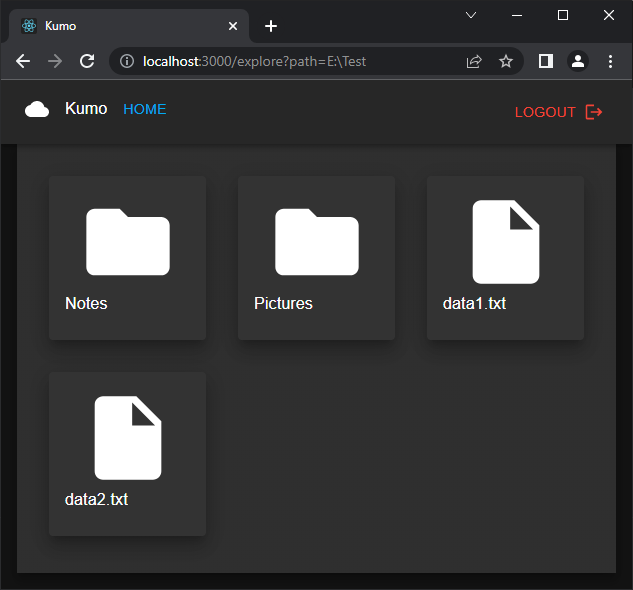
\includegraphics[scale=0.65]{./figures/chapter4/permission_manager_result.png}
	\caption{Permission manager result in the explorer}
	\label{FigPermissionManagerResult}
\end{figure}